\documentclass[xcolor=table]{beamer}
%------------------------------------------------------------
% Theme and Appearance
%------------------------------------------------------------
\usetheme[footline=authorinstitutetitle]{Berlin} 
% \usecolortheme{default}
\setbeamertemplate{navigation symbols}{} 
% Headline with Access Code
\setbeamertemplate{headline}{
    \begin{beamercolorbox}[wd=\paperwidth,ht=2.5ex,dp=1ex,right]{section in head/foot}
        \usebeamerfont{section in head/foot}
        \hspace{0.5cm}
        \ifnum\insertframenumber<30
            \raisebox{-1pt}[0pt][0pt]{\normalsize\textbf{Attendance Code: 927142}}
        \fi
        \hspace{0.5cm}
    \end{beamercolorbox}
}
% Footline with page numbers
\setbeamertemplate{footline}{
    \leavevmode%
    \hbox{%
        \begin{beamercolorbox}[wd=.333333\paperwidth,ht=2.25ex,dp=1ex,left]{author in head/foot}%
            \usebeamerfont{author in head/foot}\hspace*{0.5em}\insertshortauthor
        \end{beamercolorbox}%
        \begin{beamercolorbox}[wd=.333333\paperwidth,ht=2.25ex,dp=1ex,center]{title in head/foot}%
            \usebeamerfont{title in head/foot}\insertshorttitle
        \end{beamercolorbox}%
        \begin{beamercolorbox}[wd=.333333\paperwidth,ht=2.25ex,dp=1ex,right]{date in head/foot}%
            \usebeamerfont{date in head/foot}\insertshortdate{}\hspace*{2em}
            \insertframenumber{} / \inserttotalframenumber\hspace*{2ex} 
        \end{beamercolorbox}}%
    \vskip0pt%
}
\usepackage[utf8]{inputenc}
\usepackage[table]{xcolor}
\usepackage{colortbl}
\usepackage{minted}
\usepackage{lmodern}
\usepackage{tgheros}
\usepackage{hyperref}
\usepackage{tikz}
\usetikzlibrary{shapes, arrows, positioning, shadows, calc, decorations.pathreplacing, arrows.meta}

% % \usepackage{tikz}÷
% \usetikzlibrary{arrows.meta, positioning, shapes.geometric, calc, decorations.pathreplacing}
\usepackage{sfmath} % Sans serif math font
\renewcommand{\familydefault}{\sfdefault} % Sans serif text


\renewcommand*\familydefault{\sfdefault}

% Agenda at the start of every section
\AtBeginSection[]
{
    \begin{frame}
        \frametitle{Agenda}
        \tableofcontents[currentsection]
    \end{frame}
}

%------------------------------------------------------------
% Title Page Information
%------------------------------------------------------------
\title[CMP9134 - Week 2]{Agile Methodologies}
\subtitle{CMP9134: Software Engineering}
\author[Francesco Del Duchetto]{Dr Francesco Del Duchetto\\Lecturer in Robotics and Autonomous Systems}
\institute[University of Lincoln]{University of Lincoln}
\date{13 February 2026}

%------------------------------------------------------------
\begin{document}

%--- TITLE FRAME ---
\begin{frame}
    \titlepage
\end{frame}

%--- AGENDA FRAME ---
\begin{frame}
    \frametitle{Today's Agenda}
    \tableofcontents
\end{frame}

%------------------------------------------------------------
\section{Agile Overview}
%------------------------------------------------------------

\begin{frame}
    \frametitle{Agile Software Development}
    \begin{block}{Definition}
        A set of methods and practices based on the values and principles expressed in the \textbf{Agile Manifesto}.
    \end{block}
    \vspace{0.5cm}
    \begin{itemize}
        \item Emphasises flexibility, continuous improvement, and high-quality results.
        \item Delivered in a collaborative environment with frequent stakeholder communication.
        \item \textbf{Popular Methodologies:} Scrum, Kanban, Extreme Programming (XP), Lean Development.
    \end{itemize}
\end{frame}

\begin{frame}[fragile]
    \frametitle{Agile vs Waterfall}
    \begin{columns}
        % Waterfall
        \column{0.4\textwidth}
        \centering
        \textbf{Waterfall}\\
        \vspace{0.2cm}
        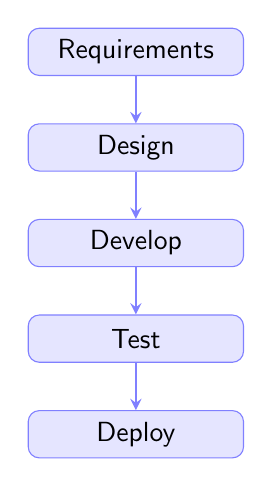
\begin{tikzpicture}[
            node distance=0.6cm,
            process/.style={rectangle, draw=blue!50, fill=blue!10, text width=2.5cm, align=center, minimum height=0.6cm, rounded corners},
            arrow/.style={->, >=stealth, thick, color=blue!50}
        ]
            \node[process] (req) {Requirements};
            \node[process, below=of req] (des) {Design};
            \node[process, below=of des] (dev) {Develop};
            \node[process, below=of dev] (test) {Test};
            \node[process, below=of test] (dep) {Deploy};
            
            \draw[arrow] (req) -- (des);
            \draw[arrow] (des) -- (dev);
            \draw[arrow] (dev) -- (test);
            \draw[arrow] (test) -- (dep);
        \end{tikzpicture}

        % Agile
        \column{0.6\textwidth}
        \centering
        \textbf{Agile}\\
        \vspace{0.2cm}
        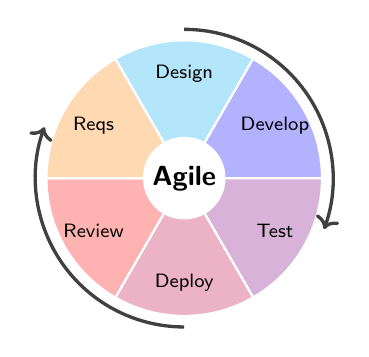
\begin{tikzpicture}[scale=0.7]
            \def\router{2.5}
            \def\rinner{1.2}
            
            % Segments
            \foreach \a/\t/\c in {
                90/Design/cyan!30,
                30/Develop/blue!30,
                -30/Test/violet!30,
                -90/Deploy/purple!30,
                -150/Review/red!30,
                150/Reqs/orange!30
            } {
                \draw[fill=\c, draw=white, thick] (0,0) -- (\a-30:\router) arc (\a-30:\a+30:\router) -- cycle;
                \node at (\a:1.9) {\scriptsize \t};
            }
            \node[circle, fill=white, inner sep=2pt] at (0,0) {\textbf{Agile}};
            
            % Cyclic arrows
            \draw[->, very thick, darkgray] (0, 2.7) arc (90:-20:2.7);
            \draw[->, very thick, darkgray] (0, -2.7) arc (-90:-200:2.7);
        \end{tikzpicture}
    \end{columns}
\end{frame}

\begin{frame}
    \frametitle{The Agile Manifesto}
    Created in February 2001 at Snowbird, Utah, by 17 software developers looking for an alternative to documentation-driven, heavyweight software development processes.
    
    \vspace{0.5cm}
    \begin{center}
        \textit{"We are uncovering better ways of developing software by doing it and helping others do it."}
    \end{center}

    \vspace{1cm}
    \begin{itemize}
        \item Manifesto: \url{https://agilemanifesto.org/}
    \end{itemize}
    
\end{frame}

\begin{frame}
    \frametitle{The Four Core Values}
    \begin{enumerate}
        \item \textbf{Individuals and interactions} over processes and tools. \\ \textit{Collaboration $>$ bureaucracy.}
        \item \textbf{Working software} over comprehensive documentation. \\ \textit{Value delivered $>$ paper trails.}
        \item \textbf{Customer collaboration} over contract negotiation.\\ \textit{Cooperation $>$ legalities.}
        \item \textbf{Responding to change} over following a plan. \\ \textit{Adaptability $>$ rigidity.}
    \end{enumerate}
    \vspace{0.3cm}
    \small \textit{That is, while there is value in the items on the right, we value the items on the left more.}
\end{frame}

\begin{frame}
    \frametitle{The Twelve Principles (Summary)}
    \footnotesize
    \begin{columns}
        \column{0.5\textwidth}
        \begin{enumerate}
            \item Customer satisfaction through early/continuous delivery.
            \item Welcome changing requirements, even late in development.
            \item Deliver working software frequently.
            \item Business people and developers work together daily.
            \item Build projects around motivated individuals.
            \item Face-to-face conversation is most efficient.
        \end{enumerate}
        
        \column{0.5\textwidth}
        \begin{enumerate}
            \setcounter{enumi}{6}
            \item Working software is the primary measure of progress.
            \item Sustainable development (constant pace).
            \item Continuous attention to technical excellence.
            \item Simplicity (maximising work \textit{not} done) is essential.
            \item Self-organising teams generate best architectures.
            \item Regular reflection and tuning of behaviour.
        \end{enumerate}
    \end{columns}
\end{frame}

\begin{frame}[fragile]
    \frametitle{Iterative vs Incremental}
    \centering
\definecolor{myblue}{RGB}{100, 110, 235}
\definecolor{myfill}{RGB}{100, 110, 235}
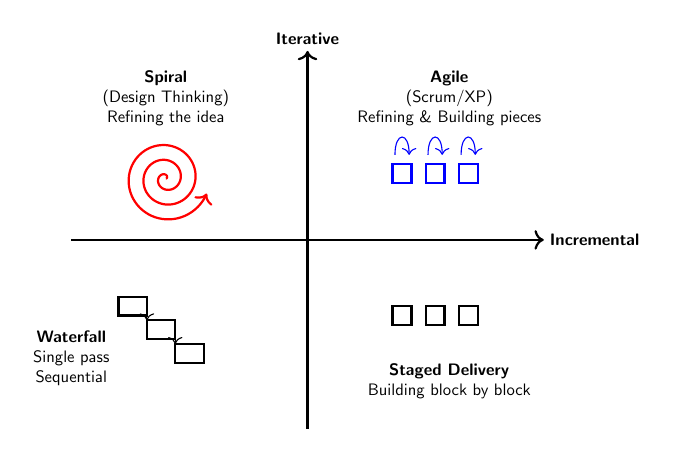
\begin{tikzpicture}[scale=0.6, transform shape]
    % --- Axes ---
    \draw[->, thick] (-5,0) -- (5,0) node[right] {\textbf{Incremental}};
    \draw[->, thick] (0,-4) -- (0,4) node[above] {\textbf{Iterative}};

    % --- Top Left: Spiral (Design Thinking) ---
    \node[align=center] at (-3, 3) {\textbf{Spiral}\\(Design Thinking)\\Refining the idea};
    
    % The Spiral Fix: Using a mathematical plot instead of a circle
    \draw[red, thick, ->] 
        plot[domain=0:18.5, variable=\t, samples=200, smooth] 
        ({-3 + 0.05*\t*cos(\t r)}, {1.3 + 0.05*\t*sin(\t r)});

    % --- Top Right: Agile (Scrum/XP) ---
    \node[align=center] at (3, 3) {\textbf{Agile}\\(Scrum/XP)\\Refining \& Building pieces};
    
    % Agile Boxes with Loops
    \foreach \x in {1.8, 2.5, 3.2} {
        % The 2D Box
        \draw[blue, thick] (\x, 1.2) rectangle ++(0.4, 0.4);
        % The Loop on top
        \draw[blue, thin, ->] (\x+0.05, 1.8) .. controls (\x+0.05, 2.3) and (\x+0.35, 2.3) .. (\x+0.35, 1.8);
    }

    % --- Bottom Left: Waterfall ---
    \node[align=center] at (-5, -2.5) {\textbf{Waterfall}\\Single pass\\Sequential};
    % Simple 2D cascading steps
    \foreach \i in {0, 1, 2} {
        \draw[thick] (-4 + \i*0.6, -1.2 - \i*0.5) rectangle ++(0.6, -0.4);
        % Small arrow between steps
        \ifnum\i<2
            \draw[->, thin] (-3.4 + \i*0.6, -1.4 - \i*0.5) -- (-3.4 + \i*0.6, -1.7 - \i*0.5);
        \fi
    }

    % --- Bottom Right: Staged Delivery ---
    \node[align=center] at (3, -3) {\textbf{Staged Delivery}\\Building block by block};
    % Simple 2D blocks
    \foreach \x in {1.8, 2.5, 3.2} 
        \draw[black, thick] (\x, -1.8) rectangle ++(0.4, 0.4);

\end{tikzpicture}
    
    \vspace{0.5cm}
    \small
    \begin{itemize}
        \item \textbf{Iterative:} Refining the solution through repeated cycles (Moving from vague to concrete).
        \item \textbf{Incremental:} Building the solution piece by piece (Adding features).
        \item \textbf{Agile} is both Iterative and Incremental.
    \end{itemize}
\end{frame}

\begin{frame}
    \frametitle{Agile Pros and Cons}
    \begin{columns}
        \column{0.5\textwidth}
        \begin{block}{Advantages}
            \begin{itemize}
                \item Flexibility and Adaptability
                \item Customer Satisfaction
                \item Improved Quality
                \item Risk Management
                \item Higher Productivity
                \item Enhanced Communication
            \end{itemize}
        \end{block}

        \column{0.5\textwidth}
        \begin{alertblock}{Disadvantages}
            \begin{itemize}
                \item Less Predictability
                \item Requires high Customer Involvement
                \item Resource Intensive (Senior talent)
                \item Scope Creep
                \item Steep Learning Curve
            \end{itemize}
        \end{alertblock}
    \end{columns}
\end{frame}

\begin{frame}
    \frametitle{Project Suitability}
    \begin{columns}
        \column{0.5\textwidth}
        \textbf{Suited for Agile:}
        \begin{itemize}
            \item Projects with uncertain/evolving requirements.
            \item Rapid delivery requirements.
            \item Innovative/Creative projects.
            \item Customer-centric products.
        \end{itemize}

        \column{0.5\textwidth}
        \textbf{Less Suitable:}
        \begin{itemize}
            \item Rigid regulatory requirements.
            \item Projects where change is costly/dangerous.
            \item Massive legacy projects difficult to break down.
            \item Fixed-price, fixed-scope contracts.
        \end{itemize}
    \end{columns}
\end{frame}

\begin{frame}
    \frametitle{Agile Success}
    % \begin{columns}
        % \column{0.5\textwidth}
        % \begin{itemize}
        %     \item User Stories
        %     \item Spikes \& Refactoring
        %     \item Pair Programming
        %     \item Test-Driven Development (TDD)
        %     \item Continuous Integration
        %     \item Collective Code Ownership
        % \end{itemize}

        % \column{0.5\textwidth}
        \centering
        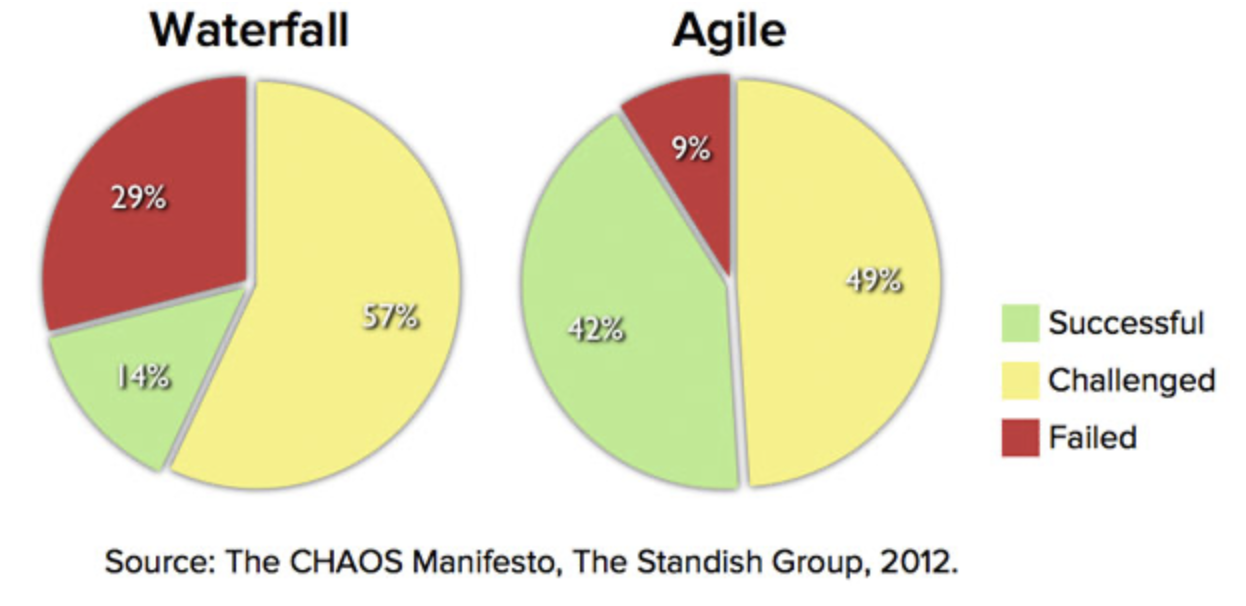
\includegraphics[width=0.8\textwidth]{agilestat.png}

        Agile projects are roughly 2X more likely to succeed than Waterfall projects, and Waterfall projects are 3X more likely to fail completely.
    % \end{columns}
\end{frame}


%------------------------------------------------------------
\section{Extreme Programming (XP)}
%------------------------------------------------------------

\begin{frame}
    \frametitle{Extreme Programming (XP)}
    Introduced in the late 1990s by Kent Beck.
    \begin{itemize}
        \item Focuses on continuous feedback and customer involvement.
        \item Emphasises technical excellence and good programming practices.
        \item Taking good practices (like testing and reviewing) to the "extreme".
    \end{itemize}
\end{frame}

\begin{frame}[fragile]
    \frametitle{XP Feedback Loops}
    \centering
    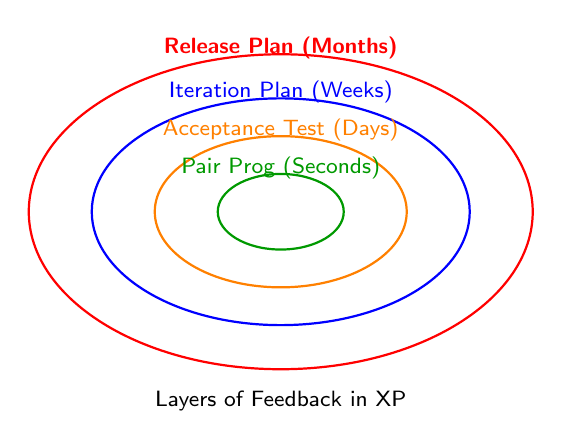
\begin{tikzpicture}[
        scale=0.8,
        every node/.style={align=center, font=\footnotesize}
    ]
        \draw[->, thick, red] (0,0) ellipse (4cm and 2.5cm);
        \node[red] at (0, 2.6) {\textbf{Release Plan (Months)}};
        
        \draw[->, thick, blue] (0,0) ellipse (3cm and 1.8cm);
        \node[blue] at (0, 1.9) {Iteration Plan (Weeks)};
        
        \draw[->, thick, orange] (0,0) ellipse (2cm and 1.2cm);
        \node[orange] at (0, 1.3) {Acceptance Test (Days)};
        
        \draw[->, thick, green!60!black] (0,0) ellipse (1cm and 0.6cm);
        \node[green!60!black] at (0, 0.7) {Pair Prog (Seconds)};
        
        \node at (0, -3) {Layers of Feedback in XP};
    \end{tikzpicture}
\end{frame}

\begin{frame}
    \frametitle{XP Roles}
    \begin{itemize}
        \item \textbf{Customer:} Defines user stories, provides acceptance criteria, responsible for business value.
        \item \textbf{Developer:} Writes code, tests, and collaborates via pair programming.
        \item \textbf{Tracker:} Tracks progress (velocity), bugs, and issues. Ensures the team is on target.
        \item \textbf{Coach:} Guides the team in XP methodology, facilitates meetings, and helps resolve conflicts.
    \end{itemize}
\end{frame}

% add new slide with image here w2/What-is-Extreme-Programming-(XP).webp
\begin{frame}
    \frametitle{XP Core Practices}
    % \begin{columns}
        % \column{0.5\textwidth}
        % \begin{itemize}
        %     \item User Stories
        %     \item Spikes \& Refactoring
        %     \item Pair Programming
        %     \item Test-Driven Development (TDD)
        %     \item Continuous Integration
        %     \item Collective Code Ownership
        % \end{itemize}

        % \column{0.5\textwidth}
        \centering
        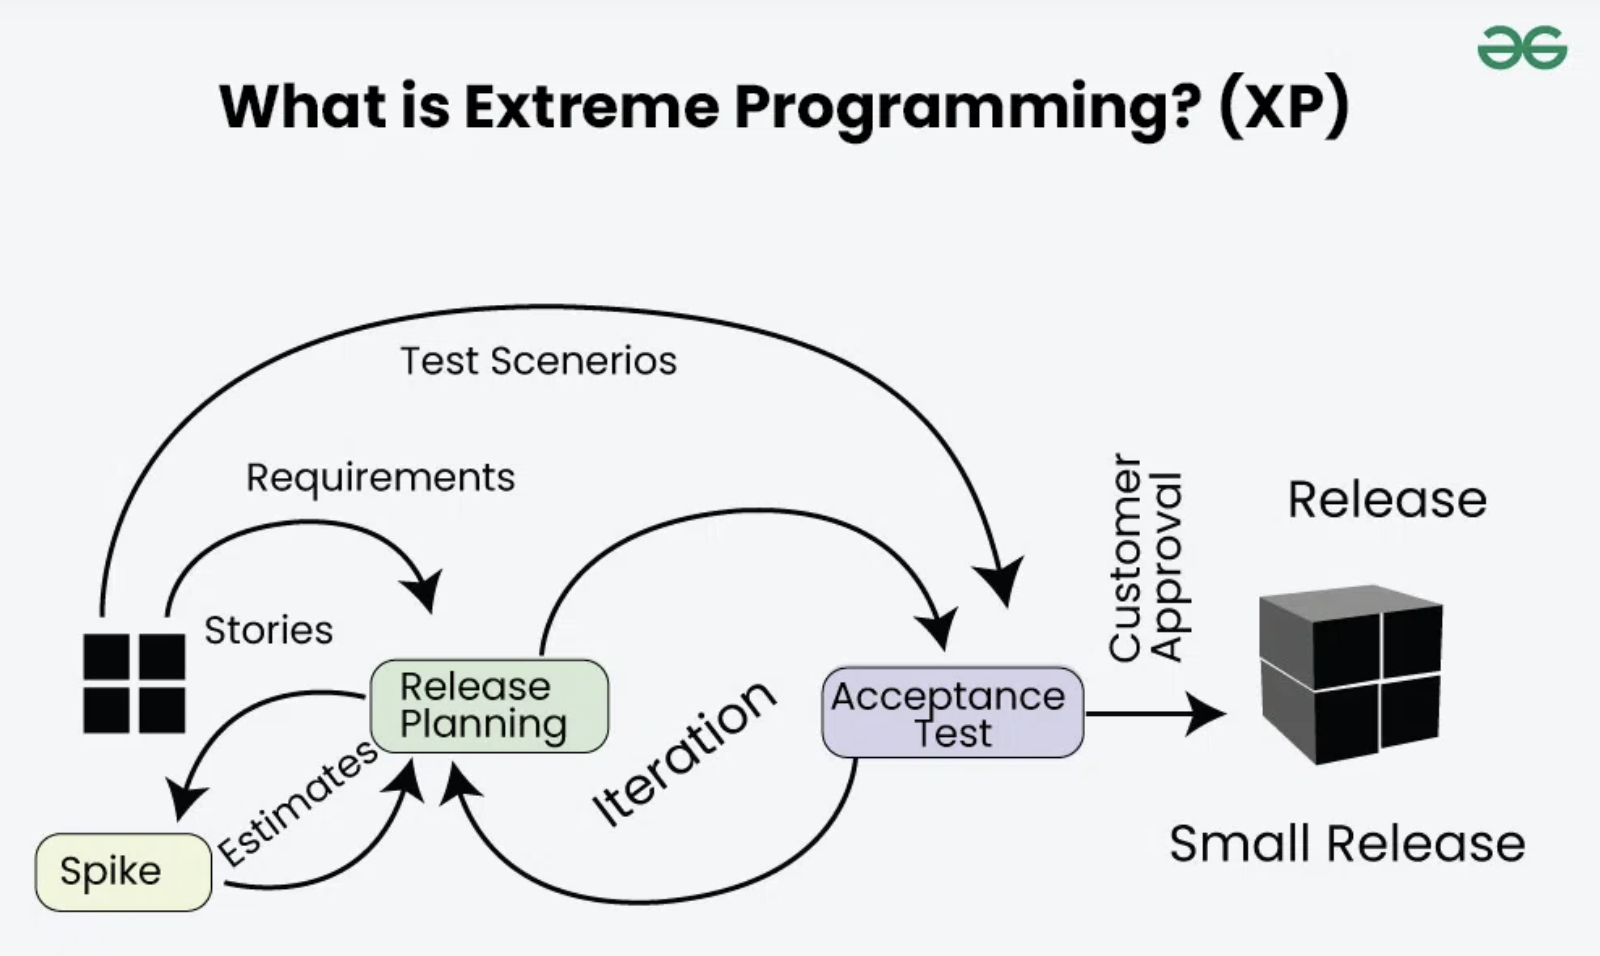
\includegraphics[width=0.8\textwidth]{Screenshot 2026-02-13 at 08.25.42.png}
    % \end{columns}
\end{frame}


\begin{frame}
    \frametitle{XP Core Practices: User Stories}
    \begin{block}{The Tool}
        A short, simple description of a feature told from the perspective of the person who desires the new capability.
    \end{block}
    
    \vspace{0.5cm}
    \textbf{Standard Format:}
    \begin{center}
        \large "As a \textcolor{red}{\textbf{$<$role$>$}}, I want to \textcolor{blue}{\textbf{$<$action$>$}}, so that \textcolor{green}{\textbf{$<$benefit$>$}}."
    \end{center}
    
    \vspace{0.3cm}
    \textbf{Example:}
    "As a \textit{registered user}, I want to \textit{view my order history}, so that \textit{I can track my purchases}."
\end{frame}

\begin{frame}
    \frametitle{XP Core Practices: Spikes \& Refactoring}
    \begin{columns}
        \column{0.5\textwidth}
        \textbf{Spike}
        \begin{itemize}
            \item A task aimed at answering a question or gathering information rather than producing shippable code.
            \item Used when estimates are uncertain due to technical unknowns.
            \item "Architectural Spike" vs "Risk-based Spike".
        \end{itemize}

        \column{0.5\textwidth}
        \textbf{Refactoring}
        \begin{itemize}
            \item Restructuring existing code without changing its external behaviour.
            \item Improves non-functional attributes (readability, reduced complexity).
            \item Essential in XP to keep the design simple as features are added.
        \end{itemize}
    \end{columns}
\end{frame}

\begin{frame}
    \frametitle{XP Core Practices: Pair Programming}
    \begin{columns}
        \column{0.6\textwidth}
        Two programmers working on a single machine.
        \begin{itemize}
            \item \textbf{The Driver:} Writes the code. Focuses on the current line of code/tactics.
            \item \textbf{The Navigator:} Reviews the code as it is typed. Focuses on strategy, bugs, and overall design.
        \end{itemize}
        \textit{Roles switch frequently.}
        
        \column{0.4\textwidth}
        \centering
        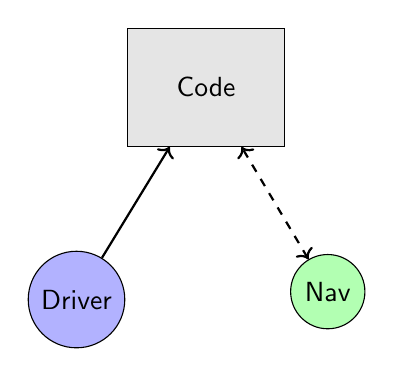
\begin{tikzpicture}
            \node[draw, rectangle, fill=gray!20, minimum width=2cm, minimum height=1.5cm] (screen) {Code};
            \node[circle, draw, fill=blue!30, below left=1.5cm and 0.2cm of screen] (p1) {Driver};
            \node[circle, draw, fill=green!30, below right=1.5cm and 0.2cm of screen] (p2) {Nav};
            \draw[->, thick] (p1) -- (screen);
            \draw[<->, dashed, thick] (p2) -- (screen);
        \end{tikzpicture}
    \end{columns}
\end{frame}


\begin{frame}
    \frametitle{XP Core Practices: Test-Driven Development (TDD)}
    \begin{block}{Definition}
        A software development process where you write tests before writing the code that implements the functionality.
    \end{block}
    
    \vspace{0.5cm}
    \textbf{The TDD Cycle:}
    \begin{center}
        \textbf{Red} $\rightarrow$ Write a failing test.\\
        \textbf{Green} $\rightarrow$ Write just enough code to pass the test.\\
        \textbf{Refactor} $\rightarrow$ Clean up the code while keeping tests green.
    \end{center}
\end{frame}

%------------------------------------------------------------
\section{Scrum}
%------------------------------------------------------------

\begin{frame}
    \frametitle{Scrum Framework}
    Scrum is an agile framework that helps teams work together. It encourages teams to learn through experiences, self-organise while working on a problem, and reflect on their wins and losses.
    
    \vspace{0.5cm}
    \begin{itemize}
        \item \textbf{Sprints:} Fixed length iterations (usually 1-4 weeks).
        \item \textbf{Artifacts:} Product Backlog, Sprint Backlog, Increment.
        \item \textbf{Roles:} Product Owner, Scrum Master, Development Team.
    \end{itemize}
\end{frame}

\begin{frame}[fragile]
    \frametitle{The Scrum Cycle}
    \centering
    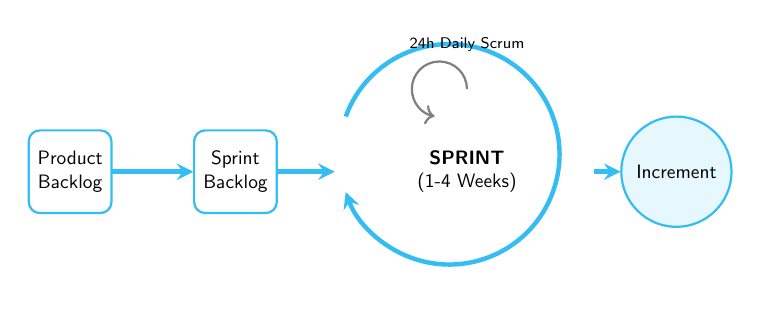
\begin{tikzpicture}[scale=0.7, transform shape,
        box/.style={rectangle, draw=cyan!80, fill=white, thick, align=center, minimum width=1.5cm, minimum height=1.5cm, rounded corners},
        circlebox/.style={circle, draw=cyan!80, fill=cyan!10, thick, align=center, minimum size=2cm},
        arrow/.style={->, >=stealth, ultra thick, cyan!80}
    ]
        % Artifacts
        \node[box] (pb) at (-6, 0) {Product\\Backlog};
        \node[box] (sb) at (-3, 0) {Sprint\\Backlog};
        
        % Sprint Cycle
        \draw[arrow] (-1, 1) arc (160:-160:2cm);
        \node[align=center] at (1.2, 0) {\textbf{SPRINT}\\(1-4 Weeks)};
        
        % Daily Scrum
        \draw[->, thick, gray] (1.2, 1.5) arc (0:260:0.5cm);
        \node[font=\footnotesize] at (1.2, 2.3) {24h Daily Scrum};

        % Output
        \node[circlebox] (inc) at (5, 0) {Increment};
        
        % Arrows
        \draw[arrow] (pb) -- (sb);
        \draw[arrow] (sb) -- (-1.2, 0);
        \draw[arrow] (3.5, 0) -- (inc);

    \end{tikzpicture}
\end{frame}

\begin{frame}
    \frametitle{Scrum Roles}
    \begin{block}{Product Owner (PO)}
        Represents stakeholders. Defines project goals, manages and prioritises the Product Backlog. Ensures value delivery.
    \end{block}
    
    \begin{block}{Scrum Master}
        Facilitates the Scrum process. Removes impediments (blockers). Protects the team from external interference. Coach and guide.
    \end{block}
    
    \begin{block}{Development Team}
        Cross-functional, self-organising group. They do the work (design, code, test) to deliver the Increment.
    \end{block}
\end{frame}

\begin{frame}
    \frametitle{Scrum Events}
    \begin{itemize}
        \item \textbf{Sprint Planning:} Team selects items from the Product Backlog to commit to for the Sprint.
        \item \textbf{Daily Scrum (Stand-up):} 15-minute sync. "What did I do yesterday? What will I do today? Blockers?"
        \item \textbf{Sprint Review:} Demo the work to stakeholders. Gather feedback.
        \item \textbf{Sprint Retrospective:} Team reflects on the process. "What went well? What can be improved?"
    \end{itemize}
\end{frame}

\begin{frame}
    \frametitle{Scrum Artifacts}
    \begin{enumerate}
        \item \textbf{Product Backlog:} An ordered list of everything needed in the product. Dynamic and prioritized by value.
        \item \textbf{Sprint Backlog:} The subset of items selected for a specific Sprint, plus the plan to deliver them.
        \item \textbf{Increment:} The sum of all backlog items completed during a Sprint + value of previous sprints. Must be "Done" (usable).
    \end{enumerate}
\end{frame}

\begin{frame}
    \frametitle{XP vs Scrum}
    \rowcolors{2}{gray!40}{white}
    \begin{table}
        \centering
        \begin{tabular}{|p{0.45\textwidth}|p{0.45\textwidth}|}
            \hline
            \textbf{XP} & \textbf{Scrum} \\
            \hline
            Iterations typically 1-2 weeks & Sprints typically 2-4 weeks \\
            Changes allowed within iteration if swapped & Scope is fixed during Sprint \\
            Strict engineering practices (TDD, Pair Programming) are mandatory & Focuses on management framework; engineering practices are optional \\
            Feedback via Code/Tests & Feedback via Review/Retro \\
            \hline
        \end{tabular}
    \end{table}
\end{frame}

%------------------------------------------------------------
\section{Agile for Solo Projects}
%------------------------------------------------------------

\begin{frame}
    \frametitle{Can Agile work for One Person?}
    \begin{block}{The "Personal Scrum" Concept}
        Agile is not limited to teams. "Personal Agility" applies the same values to manage individual workload and stress.
    \end{block}
    \vspace{0.5cm}
    \textbf{The Solo Developer wears three hats:}
    \begin{enumerate}
        \item \textbf{Product Owner:} You decide \textit{what} to build next based on value.
        \item \textbf{Scrum Master:} You ensure you are working effectively and removing distractions.
        \item \textbf{Development Team:} You do the design, coding, and testing.
    \end{enumerate}
\end{frame}

\begin{frame}[fragile]
    \frametitle{Adapting the Cycle for Solo Dev}
    \centering
    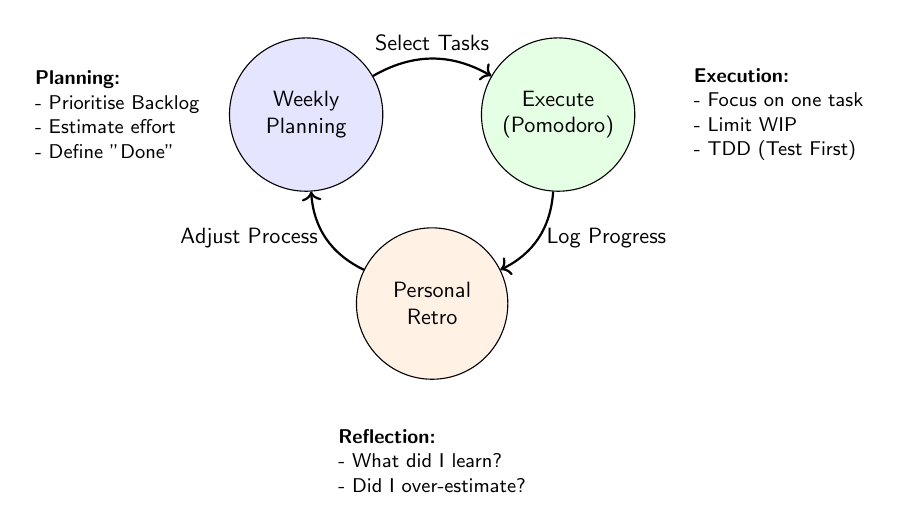
\begin{tikzpicture}[scale=0.8, transform shape]
        % Nodes
        \node[draw, circle, fill=blue!10, text width=2cm, align=center] (plan) at (0, 3) {Weekly\\Planning};
        \node[draw, circle, fill=green!10, text width=2cm, align=center] (do) at (4, 3) {Execute\\(Pomodoro)};
        \node[draw, circle, fill=orange!10, text width=2cm, align=center] (review) at (2, 0) {Personal\\Retro};
        
        % Arrows
        \draw[->, thick, bend left] (plan) to node[above] {Select Tasks} (do);
        \draw[->, thick, bend left] (do) to node[right] {Log Progress} (review);
        \draw[->, thick, bend left] (review) to node[left] {Adjust Process} (plan);
        
        % Annotations
        \node[align=left, font=\small] at (7.5, 3) {\textbf{Execution:}\\- Focus on one task\\- Limit WIP\\- TDD (Test First)};
        \node[align=left, font=\small] at (-3, 3) {\textbf{Planning:}\\- Prioritise Backlog\\- Estimate effort\\- Define "Done"};
        \node[align=left, font=\small] at (2, -2.5) {\textbf{Reflection:}\\- What did I learn?\\- Did I over-estimate?};
    \end{tikzpicture}
\end{frame}

\begin{frame}
    \frametitle{Practical Practices for Students}
    \begin{itemize}
        \item \textbf{Micro-Sprints:} Instead of 2-4 weeks, run 1-week sprints to get faster feedback on your progress.
        \item \textbf{Daily Self-Standup:} Start your day by writing down:
        \begin{itemize}
            \item What did I finish yesterday?
            \item What will I focus on today?
            \item Am I stuck? (If yes, ask a tutor/peer immediately).
        \end{itemize}
        \item \textbf{Personal Kanban:} Use Trello or GitHub Projects.
        \begin{itemize}
            \item Columns: \textit{Backlog} $\rightarrow$ \textit{This Week} $\rightarrow$ \textit{Doing (Max 1)} $\rightarrow$ \textit{Done}.
        \end{itemize}
        \item \textbf{Definition of Done:} Don't move a card to "Done" until it works and is committed to Git.
    \end{itemize}
\end{frame}

\begin{frame}
    \frametitle{Resources}
    \small
    \textbf{Academic \& Practitioner Resources for Solo Agile:}
    \vspace{0.2cm}
    \begin{itemize}
        \item \textbf{
        \href{https://files01.core.ac.uk/download/pdf/213561322.pdf}{"Personal Extreme Programming - An Agile Process for Autonomous Developers"}} (Research article). Adapts XP practices like TDD and Refactoring for solo use.
        \item \textbf{
        \href{https://www.agilesherpas.com/blog/going-agile-alone}{"Going Agile on your own"}} (Blog post). A detailed guide on shifting from "mindless productivity" to effectiveness.
        \item \textbf{
        \href{https://chrisisagile.com/personal-scrum-guide/}{"The Personal Scrum Guide"}} (Blog post). A framework specifically designed for individual freelancers and students.
        \item \textbf{
        \href{https://annas-archive.li/md5/69aa40c50001a4197b993ec0f5a52f53}{"Personal Kanban: Mapping Work - Navigating Life"}} (Book). Focuses on visualizing work to reduce cognitive load.
    \end{itemize}
\end{frame}

%------------------------------------------------------------
\section{Next Steps}
%------------------------------------------------------------

\begin{frame}
    \frametitle{Reading \& Workshop}
    \begin{itemize}
        \item \textbf{Recommended Reading:} 
        Sommerville, \textit{Software Engineering 9th Edition}, Chapter 2 (Software Processes) \& Chapter 3 (Agile).
        \item \textbf{Workshop This Week:}
        Setting up your Scrum project using \textbf{Trello}.
        \item \textbf{Next Week:}
        Software Requirements (Gathering, Analysis, Specification).
    \end{itemize}
\end{frame}

\begin{frame}
    \frametitle{Q \& A}
    \begin{center}
        \Huge Any Questions?\\\vspace{0.5cm} 
        \normalsize fdelduchetto@lincoln.ac.uk
    \end{center}
\end{frame}

\end{document}